\documentclass[11pt,titlepage,fleqn]{article}

\usepackage{amsmath}
\usepackage{amssymb}
\usepackage{latexsym}
\usepackage[round]{natbib}
\usepackage{xspace}
\usepackage{graphicx}
%\usepackage{epsfig}

\usepackage{pifont}   % search for \ding

%\usepackage{fancyhdr}
%\pagestyle{fancy}

%=====================================================
%       SPACING COMMANDS (Latex Companion, p. 52)
%=====================================================

\usepackage{setspace}

%---------------------------
\newcommand{\matlab}{\textsc{Matlab}\xspace}
%---------------------------
\renewcommand{\baselinestretch}{1.0}

\textwidth 460pt
\textheight 700pt
\oddsidemargin 0pt
\evensidemargin 0pt

% see Latex Companion, p. 85
\voffset     -50pt
\topmargin     0pt
\headsep      20pt
\headheight    0pt
\footskip     30pt
\hoffset       0pt

\include{carlcommands}
%\input{dp_header}

\graphicspath{
  {/home/vipul/REPOSITORIES/IITR_seismo/classes/ES510/latex/figures/}
  }

\begin{document}

\noindent Course: Numerical Methods and Computer Programming\\
\noindent Code: ES 510\\
\noindent Instructor: Vipul Silwal (\verb+vsilwalfes@iitr.ac.in+) \\ 
\noindent Last Compiled: \today \\

{\huge Introduction to Programming}

 \tableofcontents 
%% ------------------------------------------------------------------------ %%
\begin{section}{Types of Programming Languages}
\verb+reference: https://notes.tyrocity.com/types-of-programming-languages/+


There are two types of programming languages, which can be categorized into the following ways:
\begin{enumerate}
\item  Low level language
\begin{enumerate}
\item  Machine language (1GL)
\item  Assembly language (2GL)
\end{enumerate}
\item  High level language
\begin{enumerate}
\item  Procedural-Oriented language (3GL)
\item  Problem-Oriented language (4GL)
\item  Natural language (5GL)
\end{enumerate}
\end{enumerate}

\iffalse
\begin{enumerate}
 \item       Low level language

This language is the most understandable language used by computer to perform its operations. It can be further categorized into:
\begin{enumerate}
\item  Machine Language (1GL)

Machine language consists of strings of binary numbers (i.e. 0s and 1s) and it is the only one language, the processor directly understands. Machine language has an Merits of very fast execution speed and efficient use of primary memory.

Merits:
\begin{itemize}
\item  It is directly understood by the processor so has faster execution time since the programs written in this language need not to be tanslated.
\item  It doesn’t need larger memory.
\end{itemize}
Demerits:
\begin{itemize}
\item It is very difficult to program using 1GL since all the instructions are to be represented by 0s and 1s.
\item Use of this language makes programming time consuming.
\item It is difficult to find error and to debug.
\item  It can be used by experts only.
\end{itemize}
\item  Assembly Language

Assembly language is also known as low-level language because to design a program programmer requires detailed knowledge of hardware specification. This language uses mnemonics code (symbolic operation code like ‘ADD’ for addition) in place of 0s and 1s. The program is converted into machine code by assembler. The resulting program is reffered to as an object code.

Merits:
\begin{itemize}
\item It is makes programming easier than 1GL since it uses mnemonics code for programming. Eg: ADD for addition, SUB for subtraction, DIV for division, etc.
\item It makes programming process faster.
\item Error can be identified much easily compared to 1GL.
\item It is easier to debug than machine language.
\end{itemize}
Demerits:
\begin{itemize}
\item Programs written in this language is not directly understandable by computer so translaters should be used.
\item It is hardware dependent language so programmers are forced to think in terms of computer’s architecture rather than to the problem being solved.
\item Being machine dependent language, programs written in this language are very less or not protable.
\item Programmers must know its mnemonics codes to perform any task.
\end{itemize}
\end{enumerate}
\item       High level language

Instructions of this language closely resembles to human language or English like words. It uses mathematical notations to perform the task. The high level language is easier to learn. It requires less time to write and is easier to maintain the errors. The high level language is converted into machine language by one of the two different languages translator programs; interpreter or compiler.

High level language can be further categorized as:
\begin{enumerate}
\item  Procedural-Oriented language (3GL)

Procedural Programming is a methodology for modeling the problem being solved, by determining the steps and the order of those steps that must be followed in order to reach a desired outcome or specific program state. These languages are designed to express the logic and the procedure of a problem to be solved. It includes languages such as Pascal, COBOL, C, FORTAN, etc.

Merits:
\begin{itemize}
\item  Because of their flexibility, procedural languages are able to solve a variety of problems.
\item  Programmer does not need to think in term of computer architecture which makes them focused on the problem.
\item  Programs written in this language are portable.
\end{itemize}
Demerits:
\begin{itemize}
\item  It is easier but needs higher processor and larger memory.
\item  It needs to be translated therefore its execution time is more.
\end{itemize}

\item  Problem-Oriented language (4GL)

It allows the users to specify what the output should be, without describing all the details of how the data should be manupulated to produce the result. This is one step ahead from 3GL. These are result oriented and include database query language.
Eg: Visual Basic, C\#, PHP, etc.
The objectives of 4GL are to:
\begin{itemize}
\item  Increase the speed of developing programs.
\item Minimize user’s effort to botain information from computer.
\item Reduce errors while writing programs.
\end{itemize}
   Merits:
\begin{itemize}
\item  Programmer need not to think about the procedure of the program. So, programming is much easier.
\end{itemize}
Demerits:
\begin{itemize}
\item  It is easier but needs higher processor and larger memory.
\item It needs to be translated therefore its execution time is more.
\end{itemize}

\item  Natural language (5GL)

Natural language are stil in developing stage where we could write statrments that would look like normal sentences.
Merits:
\begin{itemize}
\item  Easy to program.
\item Since, the program uses normal sentences, they are easy to understand.
\item The programs designed using 5GL will have artificial intelligence (AI).
\item The programs would be much more interactive and interesting.
\end{itemize}
Demerits:
\begin{itemize}
\item It is slower than previous generation language as it should be completely translated into binary code which is a tedious task.
\item  Highly advanced and expensive electronic devices are required to run programs developed in 5GL. Therefore, it is an expensive approach.
These are the different types of programming languages with their merits and demerits.
\end{itemize}
\end{enumerate}
\end{enumerate}
\fi
\end{section}
%-----------------------------------------------------

\begin{section}{Another way of categorizing}
\verb+https://android.jlelse.eu/magic-lies-here-statically-typed-vs-dynamically-typed-languages-d151c7f95e2b+

How and when the type of the data is defined. This is could be performedduring compile of code (a static check; example: C, C++) or at run-time (dynamic, example: Python, MATLAB). 

If a language specification requires its typing rules strongly (i.e., more or less allowing only those automatic type conversions that do not lose information), one can refer to the process as Strongly typed, if not, as Weakly typed.

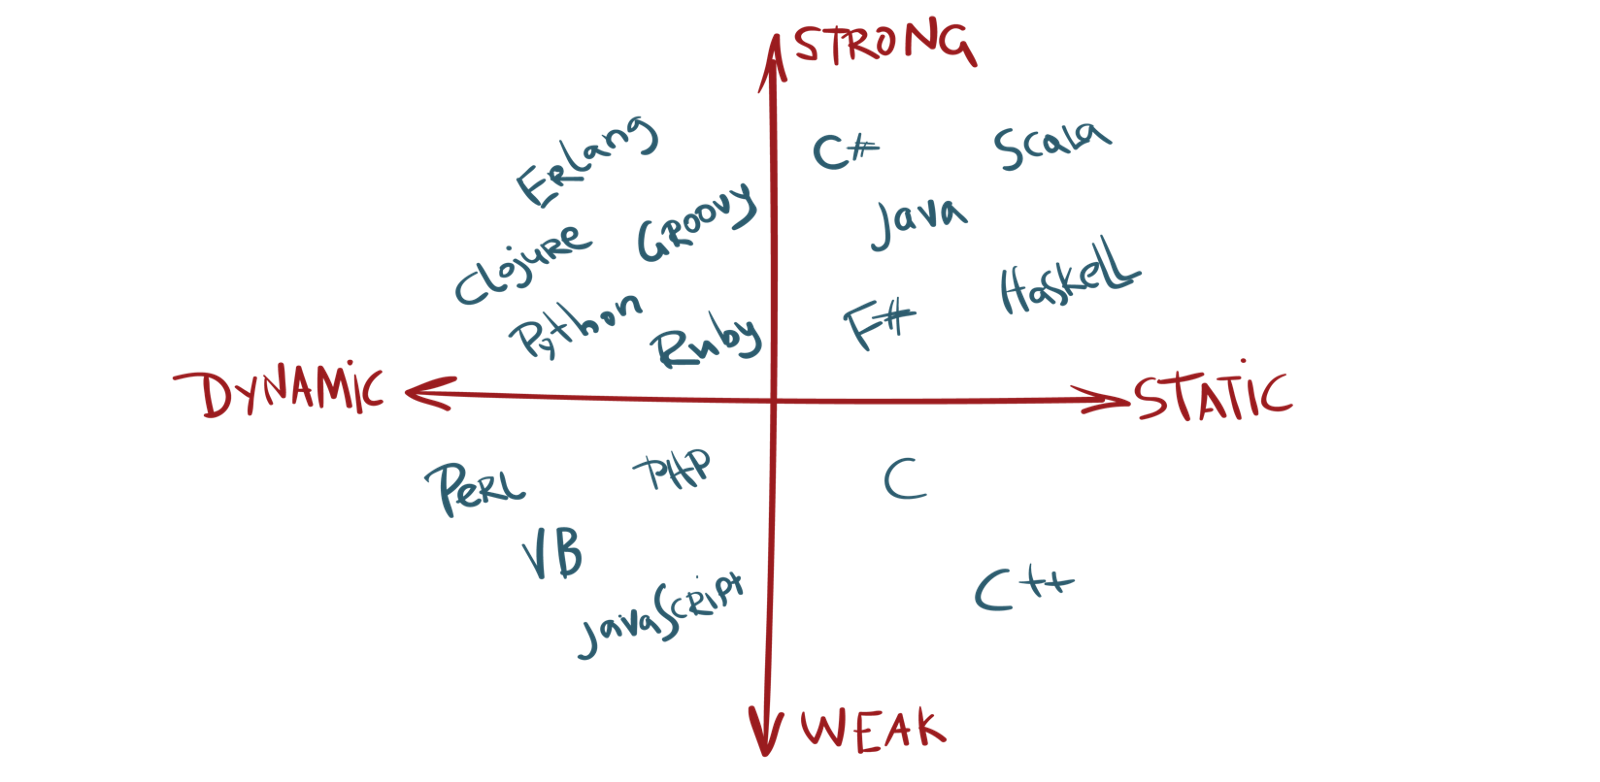
\includegraphics[scale=0.25]{data_types.png}
\end{section}
%-----------------------------------------------------

\begin{section}{Common Data Types}
\begin{enumerate}
\item Numbers
\begin{enumerate}
\item Integers \\
\begin{tabular}{|c|c|c|}
\hline
Data Type             &  	Range of Values &	Conversion Function\\
\hline
Signed 8-bit integer  & 	-2$^7$ to 2$^7$-1 &	int8\\
Signed 16-bit integer &	-2$^{15}$ to 2$^{15}$-1 &	int16\\
Signed 32-bit integer &	-2$^{31}$ to 2$^{31}$-1 &	int32\\
Signed 64-bit integer &	-2$^{63}$ to 2$^{63}$-1 &	int64\\
Unsigned 8-bit integer  &	0 to 2$^{8}$-1  &	uint8\\
Unsigned 16-bit integer &	0 to 2$^{16}$-1 &	uint16\\
Unsigned 32-bit integer	& 0 to 2$^{32}$-1 &	uint32\\
Unsigned 64-bit integer	& 0 to 2$^{64}$-1 &	uint64\\
\hline
\end{tabular}

By default \matlab would assign double precision (8 bytes)
\begin{verbatim}
>> a = 2

a =

     2

>> class(a)

ans =

    'double'
>> whos a
  Name      Size            Bytes  Class     Attributes

  a         1x1                 8  double  

\end{verbatim}

This type conversion (using commands: \verb+int8, int16, int32, int64+) could be performed depending on the values the parameter would store. For example, if you know that value value is either going to be integer only (and not decimal), then there is not point using 8 bytes variable; a simple 1 byte character would to the same job.
\begin{verbatim}
>> a=21.6

a =

   21.6000

>> a8 = int8(a)

a8 =

  int8

   22
>> whos a a8
  Name      Size            Bytes  Class     Attributes

  a         1x1                 8  double              
  a8        1x1                 1  int8 
\end{verbatim}

\begin{verbatim}


>> a = boolean(21)

a =

  logical

   1

>> whos a
  Name      Size            Bytes  Class      Attributes

  a         1x1                 1  logical  
\end{verbatim}


\item Floats\\
Decimal number, very large and very small number are represented by floating point numbers.

\begin{tabular}{|c|c|}
\hline
Bits &	Usage\\
\hline
63 &	Sign (0 = positive, 1 = negative)\\
62 to 52 &	Exponent, biased by 1023\\
51 to 0 &raction f of the number 1.f\\
\hline
\end{tabular}

\begin{verbatim}
str = 'The range for double is:\n\t%g to %g and\n\t %g to  %g';
sprintf(str, -realmax, -realmin, realmin, realmax)

ans =
The range for double is:
   -1.79769e+308 to -2.22507e-308 and
    2.22507e-308 to  1.79769e+308
\end{verbatim}

\item Complex Numbers

\begin{verbatim}
>> a = 1 + 2i;
>> whos a
  Name      Size            Bytes  Class     Attributes

  a         1x1                16  double    complex  
\end{verbatim}
\end{enumerate}

\item alphanumeric
\begin{enumerate}
\item Characters
\item Strings

\begin{verbatim}
>> a= 'a'
>> whos a
  Name      Size            Bytes  Class    Attributes

  a         1x1                 2  char  
>> a= 'ab'
>> whos a
  Name      Size            Bytes  Class    Attributes

  a         1x2                 4  char 
\end{verbatim}

\end{enumerate}
\item Boolean - O's and 1's (No and Yes)
\end{enumerate}
\end{section}
%-----------------------------------------------------

\begin{section}{Vector and Matrix Representation}
One dimensional matrices are called Vectors. In my view it is best to define vector as column vector instead of row vector, since that makes it more relatable to how we actually write it on paper (in linear algebra).

{\bf Example:} Projectile motion and quadratic equation

Standard quadratic equation is given by:
\begin{equation}
a x^2 +b x + c = 0 \label{quad}
\end{equation}

Horizontal and vertical displacement for a projectile is given by''
\begin{eqnarray}
x &=& v_0 t \cos(\theta)\\  \label{disp} 
y &=& v_0 t \sin(\theta) - \frac{1}{2} g t^2 
\end{eqnarray}

Now consider time, t, goes from 0 to 100 seconds. Let's discretize this time into 1000 points (or  999 spaces).
\verb+ t = linspace(0,100,1000)+ \\
With initial velocity, $v_0 = 500$ m/s, and inital angle as $\theta = 60^o$.

\begin{verbatim}
%% EXAMPLE: Projectile
t = linspace(0,100,1000);   % in seconds
v0 = 500;                   % in m/s
theta = 60;                 % in degrees

% constant
g = 9.8;                    % m/s2 (gravity constant)

% horizontal and vertical displacements
x = v0 * t * cosd(theta);
y = v0 * t * sind(theta) - 0.5 * g * t.^2;

% plot
plot(x,y)
\end{verbatim}

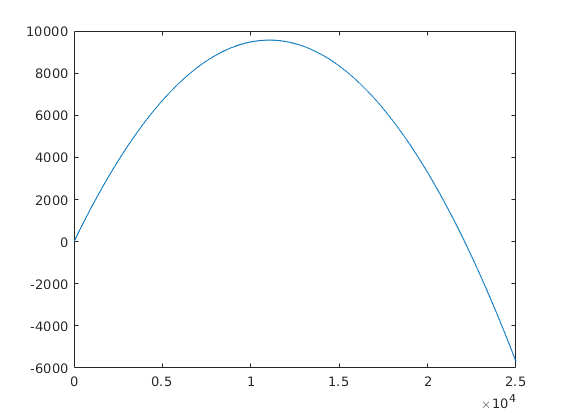
\includegraphics[scale=.8]{projectile.png}

\begin{subsection}{Convention}
There are no hard an fast rules on how the variables should be named. But 'good programming practice' calls for some sort of naming conventions so that it makes programme more readable and shareable.
Typically, scaler variables are denoted as lowercase letters and matrices are represented by uppercase letters (however, no standard convention accepted globaly).

\end{subsection}
\end{section}

\begin{section}{Operators}

{\bf Arithmetic Operators}
\begin{tabular}{|c|c|c|}
\hline
Symbol  &	Role  &	More Information \\
\hline
+  &	Addition  &	plus\\
-  &	Subtraction  &	minus\\
.*  &	Element-wise multiplication  &	times\\
*  &	Matrix multiplication  &	mtimes\\
./  &	Element-wise right division  & rdivide\\
/  &	Matrix right division  &	mrdivide\\
.\  &	Element-wise left division  &	ldivide\\
\  &	Matrix left division(also known as backslash)  &	mldivide\\
.\^ &	Element-wise power  &	power\\
\^ \ &	Matrix power  &	mpower\\
.'  &	Transpose  &	transpose\\
'  &	Complex conjugate transpose  &	ctranspose\\
\hline
\end{tabular}

{\bf Relational Operators}
\begin{tabular}{|c|c|c|}
\hline
Symbol  &	Role  &	More Information \\
\hline
== &	Equal to &	eq\\
$\sim=$ &	Not equal to &	ne\\
$>=$ &	Greater than &	gt\\
$>$ &	Greater than or equal to &	ge\\
$<$ &	Less than &	lt\\
$<=$ &	Less than or equal to & le\\
\hline
\end{tabular}

{\bf logical Operators}
\begin{tabular}{|c|c|c|}
\hline
Symbol  &	Role  &	More Information \\
\hline
\& &	Logical AND &	and\\
$|$ &	Logical OR  &	or\\
\&\& &	Logical AND (with short-circuiting) & second operand evaluated only ...\\
$||$ &	Logical OR (with short-circuiting)  & ... when first is not satisfied\\
$\sim$ &	Logical NOT &	not\\
\hline
\end{tabular}
\end{section}

\begin{section}{Reading and Writing ASCII files}
Two most used function for reading the ASCII data files are:
\begin{enumerate}
\item \verb+dlmread+

This is mainly for reading numeric data (saved in a file) into a matrix.
(Note: Recently \matlab has been suggesting \verb+readmatrix+ funtion instead).

\begin{verbatim}
ddir = '~/REPOSITORIES/IITR_seismo/classes/ES510/lab/data/';
fname = 'XZ_GOAT_BHZ.dat';
    
fid = fopen(strcat(ddir,fname));
data = dlmread(strcat(ddir,fname));
\end{verbatim}
\item \verb+textscan+ 

Allows for formatting options and reads any (char, numbers) in \matlab cell array. Headerline can also be handeled easily.

\begin{verbatim}
ddir = '~/REPOSITORIES/IITR_seismo/classes/ES510/lab/data/';
fname = 'XZ_GOAT_BHZ.dat';
    
fid = fopen(strcat(ddir,fname));
data = textscan(fid,'%f');
\end{verbatim}
\end{enumerate}
\end{section}


%-----------------------------------------------------

\begin{section}{Exercise}
\begin{enumerate}
\item Find roots of quadratic equation

Roots are the zero-crossing points, and since this is a quadratic equation, it will have two roots.  Using equations \ref{quad} -- \ref{disp}, find the zero crossing points. [Hint: All you need to find the x values for which y is 0].

\item Read and visualize waveform data

See Example 2 of the \matlab lab assignment. Find the x's where y is maximum and minimum.

\item Rotation Exercise

Rotation matrix is defined as, 
${\bf R} = 
\begin{bmatrix} 
\cos \theta & -\sin \theta \\
\sin \theta & \cos \theta
\end{bmatrix}$, 
where $\theta$ is 

\begin{equation}
{\bf M} = 
\end{equation}

\item Compute seismic moment (example of matrix dot product)

\item Read and Visualize 3D data

\end{enumerate}
\end{section}
%-----------------------------------------------------
\end{document}
